\documentclass[12pt, twoside]{article}
\usepackage[hmargin=1.25in, vmargin=1.1in]{geometry}

\usepackage[utf8]{inputenc}
\usepackage[T1]{fontenc}
\usepackage[english]{babel}
\usepackage{pdfpages}
\usepackage{listings}
\usepackage{color}
\usepackage{graphicx}
\usepackage{float}
\usepackage{hyperref}
\usepackage{url}
\usepackage{upquote}
\usepackage{lastpage}
\usepackage{fancyhdr}
\pagestyle{fancy}
\usepackage{longtable}
\usepackage{tabu}
\usepackage{rotating}
\usepackage[strings]{underscore}
\usepackage[nottoc,numbib]{tocbibind}

\graphicspath{ {images/} }

\newcommand{\helv}{\fontfamily{phv}\fontseries{b}\fontsize{9}{11}\selectfont}

%--------------- Variables à modifier à chaque rendu ---------------
\title{Data description}
\newcommand{\daterendu}{06/26/2019}
%-------------------------------------------------------------------

\makeatletter\let\Title\@title\makeatother

% Décommenter pour commencer les chapitres à 0
%\setcounter{section}{-1}

\begin{document}

\begin{titlepage}

\newcommand{\HRule}{\rule{\linewidth}{0.5mm}} % Defines a new command for the horizontal lines, change thickness here

\center % Center everything on the page



\includegraphics[width=0.8\textwidth]{logo_HEIA.jpg}

\includegraphics[width=0.3\textwidth]{logo_LBNL.png}\\[1.1cm]
\textsc{\Large Bachelor thesis \\ [0.3cm]
\large Year 2018-2019 }\\ [2.0cm]


\textsc{
\bfseries \LARGE Machine learning for noise reduction in images of old audio records}\\ [1.0cm]


\HRule \\[0.5cm]
{ \huge \bfseries \Title }\\ 
\HRule \\[1.2cm]

\Large
Benoit \textsc{Ruffray}\\[1.0cm] 

{\large Date : \daterendu}\\[1.3cm] 

\begin{flushleft}
\large External supervisor: Haber~Carl
\end{flushleft}
\begin{flushleft}
	\large Internal supervisors: Bapst~Frédéric / Hennebert~Jean
\end{flushleft}
\begin{flushleft}
\large Consultants: Cornell~Earl / Nachman~Benjamin
\end{flushleft}

\end{titlepage}
\pagenumbering{Roman}

\renewcommand{\headrulewidth}{1pt}
\fancyhead[L]{\helv ML-for-NR}
\fancyhead[C]{\helv 2018-2019}
\fancyhead[R]{\helv \Title }

\renewcommand{\footrulewidth}{1pt}
\fancyfoot[C]{\helv Table of contents \thepage{}}

\setcounter{page}{1}

\begin{center}
\tableofcontents
\end{center}

\newpage

\fancyhf{}
\renewcommand{\headrulewidth}{1pt}
\fancyhead[L]{\helv ML-for-NR}
\fancyhead[C]{\helv 2018-2019}
\fancyhead[R]{\helv \Title }

\renewcommand{\footrulewidth}{1pt}
\fancyfoot[LO, RE]{\helv Bachelor thesis, year 2018 - 2019}
\fancyfoot[C]{}
\fancyfoot[RO, LE]{\helv \textbf{Page \thepage{}/\pageref{LastPage}}}
\pagenumbering{arabic}
\setcounter{page}{1}
\section{Introduction}
This document describes the properties of the system and the data used for the Machine Learning for Noise Reduction (ML4NR) project.
\section{Architecture}
The system used by the Lawrence Berkeley National Laboratory (LBNL) for record preservation and audio reconstruction follows a simple pipeline.

IRENE (Image, Reconstruct, Erase Noise, Etc.) is a machine able to take high resolution pictures of a disc. Weaver is a software made for image processing, allowing to find edges, grooves, and playing back the carved sound.
\subsection{IRENE}
Stands for Image, Reconstruct, Erase Noise, Etc.
IRENE is a scanning machine used to image discs and cylinders. It's composed of high-resolution 2D and 3D cameras, and rotating supports for the records.

The 2D camera takes pictures of one line on the disc, 1 pixel high for thousands of pixels long. The pictures are taken at a very high frequency while the record is turning, imaging the disc line by line. The actual frequency is tuned for the support imaged.

To take pictures, light is directed with a certain angle on the disc. The sensors are activated by the reflected light, and write the perceived amount. Direct reflection results in white pixels, no light reflected becomes black, and in between are the gray scales.

%add groove and camera schema

The grooves are usually made of large white bands outside (the disc surface), black bands inside (the groove's "walls"), and a thin white and in the middle (bottom of the groove). Between these bands, there is a small area of gray scaled pixels.

%add groove example
\subsection{Weaver}
Weaver is a collection of plugins made for disc image processing. Over the years, more than a hundred plugins have been developed, such as image loading, pixel binning, edge detection, groove derivative calculation, sound construction, etc.
\section{Images of shellac discs}
Shellac discs are imaged by IRENE at a frequency of 104 KHz, and they are read at 78 RPM. This results in pictures with a height of 80 000 pixels. IRENE can image 8 to 9 grooves at the same time, for a width of 4096 pixels. Multiple pictures are necessary to image the entire disc. They are usually written in bitmap format.

So, an entire shellac disc consists of 15 to 30 pictures of dimension 4096 x 80'000, depending on the length of the track. Each line of pixels is 1/104000 of a second. 
%TODO add imaged disc
\subsection{Noise}
Most of the shellac discs images are noisy, because of the texture of the support and the disc wearing out. The noise is almost inaudible during playback, but the current algorithm for audio reconstruction is very sensitive to it. The reconstructed audio contains a high pitched background noise.

The noise can be as small as 1 pixel wide, but can also go to 10s of pixels. It's very difficult to reconstruct the missing groove, as the only information is the groove before and after. Most of the time it works by correcting the groove with a straight line, or copying the previous properties of the groove, but it's possible that there was something different before the damage came.
\section{Audio files}
The audio files will be used for setting a goal. They can be the original audio (from CD or tape), or the reconstruction made by Weaver.
\subsection{Original CD audio}
This audio file, coming from a tape or a CD, is the original audio used to print the shellac disc. It is therefore what was meant to be played. The bit rate changes for each track.
\subsection{Reconstructed audio}
The audio reconstructed form the disc images by Weaver. It contains a background noise.

The exact line where it started in the image is given in the headers.
%\begin{figure}[H]
%	\centering
%	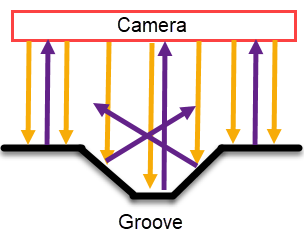
\includegraphics[width=0.5\textwidth]{grooveside.png}
%	\caption{Camera lighting the groove and detecting direct reflection}
%	\label{grooveside}
%\end{figure}

%\bibliographystyle{unsrt}
%\bibliography{cdc}
%\includepdf[pages={3}]{planV1.pdf}
\end{document}